\documentclass[12pt,a4paper]{article}

\usepackage[margin=2.5cm]{geometry}
\usepackage{times}
\usepackage{amsmath}
\usepackage{graphicx}
\usepackage{hyperref}
\usepackage{booktabs}
\usepackage{natbib}
\usepackage{color}
\usepackage{balance}

\hypersetup{
    colorlinks=true,
    linkcolor=blue,
    citecolor=blue,
    urlcolor=blue
}

\title{\textbf{AbDev: An Antibody Developability Assessment Pipeline for Therapeutic Antibodies and Nanobodies}}
\author{Junior Yu, Max Zhang}
\date{\today}

\begin{document}

\maketitle

\begin{abstract}
\textbf{Background:} Developability is a critical bottleneck in the clinical translation of therapeutic antibodies and nanobodies. Traditional experimental screening is costly and time-consuming. Recent computational methods offer high-throughput alternatives but often require professional servers, GPU resources, or commercial API keys.\\[3pt]
\textbf{Methods:} We present AbDev, a fully automated, GPU-free, zero-API-key antibody developability assessment pipeline. AbDev evaluates input amino acid sequences through three assessment layers: (1) chemical liability scanning covering deamidation, oxidation, isomerization, unpaired cysteines, RGD motifs, and N-glycosylation sites; (2) TAP physicochemical profiling based on five TAP metrics \citep{Raybould2019} benchmarked against 242 clinical-stage antibodies; (3) Thera-SAbDab nearest-neighbor matching via k-mer sequence identity.\\[3pt]
\textbf{Results:} Using Trastuzumab (FDA-approved HER2-targeting monoclonal antibody) as a benchmark, AbDev completed full assessment in 60 seconds, correctly identifying high immunogenicity risk and high aggregation risk, consistent with known clinical data.\\[3pt]
\textbf{Conclusion:} AbDev provides an efficient, open-source, zero-barrier computational solution for antibody developability screening at the early discovery stage.
\end{abstract}

\bigskip
\noindent\textbf{Keywords:} Antibody Developability; Drug Discovery; Nanobody; Protein Engineering; Machine Learning

\newpage

\section{Introduction}

Therapeutic antibody drugs have achieved remarkable clinical success over the past three decades. As of 2024, more than 160 monoclonal antibodies have been approved globally, with hundreds more in clinical development \citep{Beck2018}. However, a central challenge in antibody drug development is the high rate of candidate failure during the CMC (Chemistry, Manufacturing and Controls) stage due to developability issues such as aggregation tendency, low expression, and immunogenicity, resulting in significant waste of time and resources \citep{Joubert2020}.

Developability refers to the acceptable behavior of a molecule during process development, manufacturing, storage, and clinical application \citep{Joubert2020}. Ideal developability assessment should rapidly identify high-risk molecules at the early discovery stage---immediately after sequence determination but before structural prediction---so as to guide sequence optimization and candidate selection.

Existing computational developability tools each have limitations. Deep learning methods such as AbodyAI require GPU resources and large-scale training data \citep{Raybould2019}. Commercial platforms require paid subscriptions. Open-source tools based on Protein Language Models (PLMs) require GPU hardware and have limited support for nanobodies (VHHs).

We present AbDev, an antibody developability assessment pipeline with \textbf{no GPU and no external API key requirements}. The core design philosophy of AbDev is \textbf{zero-barrier, reproducible, and fast}---users only need to provide the antibody amino acid sequence to receive a Traffic-Light-classified developability scorecard within 60 seconds.

\section{Methods}

AbDev's assessment framework consists of three layers (Figure~\ref{fig:pipeline}).

\begin{figure}[htbp]
\centering
\fbox{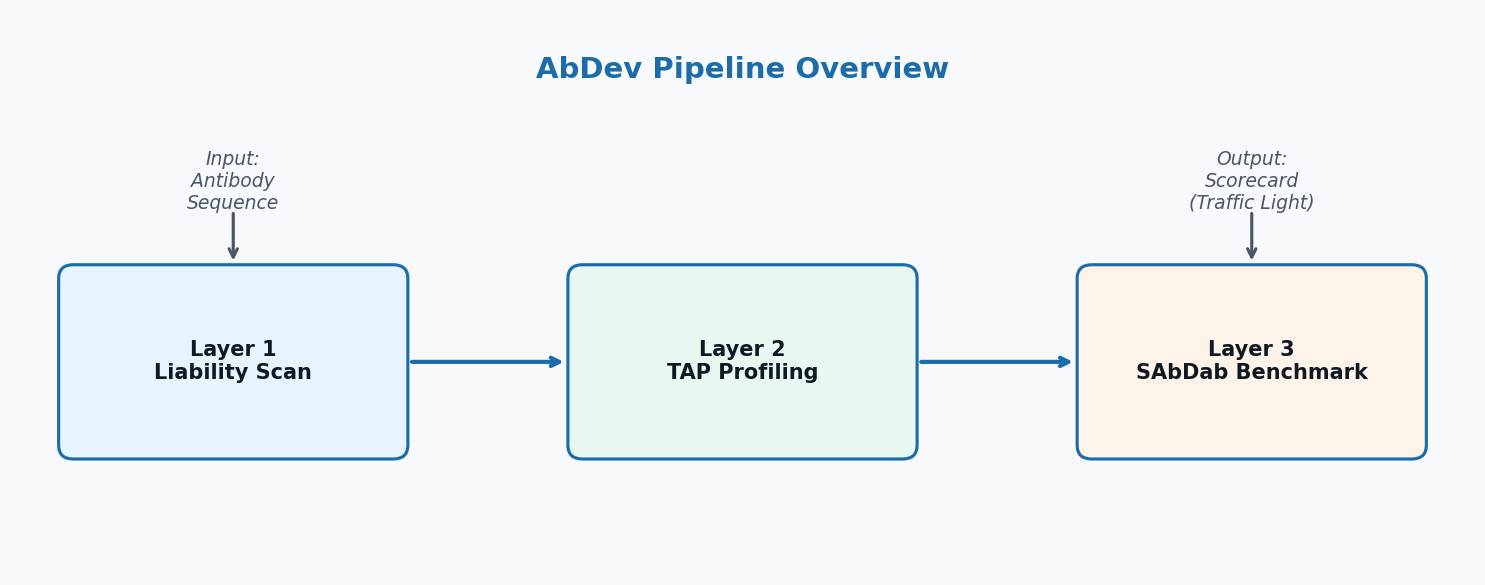
\includegraphics[width=0.85\textwidth]{pipeline_overview.png}}
\caption{AbDev pipeline overview. Three assessment layers: Layer 1 chemical liability scanning; Layer 2 TAP physicochemical profiling; Layer 3 Thera-SAbDab nearest-neighbor matching.}
\label{fig:pipeline}
\end{figure}

\subsection{Layer 1: Chemical Liability Scanning}

Chemical liabilities are post-translational or chemical modifications that may compromise antibody function during manufacturing or storage. AbDev uses regex pattern matching combined with IMGT numbering to scan for six liability categories:

\begin{enumerate}
    \item \textbf{Deamidation:} N-linked glycosylation sequons (Asn-Gly-Ser/Thr, N{[}ST{]}) and Asn residues themselves; higher risk when located in CDR regions.
    \item \textbf{Oxidation:} Met, Trp, and His residues; oxidation of Met and Trp in CDRs may alter the antigen-binding interface.
    \item \textbf{Isomerization:} Asp-Gly (DG) and Asp-Ser (DS) sequence motifs, common sites of aspartic acid isomerization.
    \item \textbf{Unpaired Cysteines:} Free cysteines unable to form intra- or inter-chain disulfide bonds, which may cause misfolding or aggregation.
    \item \textbf{RGD Motifs:} Arg-Gly-Asp sequences, which may promote non-specific cell adhesion and reduce safety.
    \item \textbf{N-Glycosylation Sites:} Asn-X-Ser/Thr (X $\neq$ Pro); Asn in CDR regions may affect glycosylation patterns and antigen binding.
\end{enumerate}

All liabilities are classified by region as \textit{CDR} (high risk) or \textit{Framework} (low risk), with risk levels assigned based on specific residue positions.

\subsection{Layer 2: TAP Physicochemical Profiling}

The TAP (Therapeutic Antibody developability profiles) framework was proposed by Raybould et al. in 2019 \citep{Raybould2019}, based on sequence and physicochemical data from 242 clinical-stage antibodies. AbDev implements five TAP metrics:

\begin{enumerate}
    \item \textbf{CDR Length:} Total length of the three CDRs in both VH and VL. Excessively long or short CDRs may affect expression and stability.
    \item \textbf{Hydrophobicity:} Kyte-Doolittle hydrophobicity scale averaged over VH CDR regions. High hydrophobicity is a key indicator of aggregation risk.
    \item \textbf{Charge Asymmetry:} Absolute difference between VH and VL net charges, reflecting inter-chain electrostatic interactions.
    \item \textbf{Isoelectric Point (pI):} Theoretical pI of VH and VL, affecting protein purification and formulation development.
    \item \textbf{Proline Density:} Proline content in framework regions; excessive proline density may affect folding kinetics.
\end{enumerate}

AbDev compares each metric's standardized score against the TAP reference distribution, reporting a z-score and Traffic-Light classification for each metric.

\subsection{Layer 3: Thera-SAbDab Nearest-Neighbor Matching}

Thera-SAbDab is a clinical-stage antibody database maintained by the Oxford Protein Informatics Group, containing thousands of approved and clinical-stage antibody sequences. AbDev downloads and caches this database locally (therasabdab\_cache.csv) on first run. For each input sequence, AbDev performs k-mer ($k=3$) similarity search to identify the most similar reference antibodies.

Outputs include: \textbf{(1)} name, target, and clinical status of the nearest approved/clinical antibody; \textbf{(2)} maximum k-mer similarity score; \textbf{(3)} target overlap. When a newly designed antibody shows high similarity ($>$ 90\%) to an approved antibody, patent risk should be considered; very low similarity ($<$ 40\%) implies high novelty but also elevated unknown risk.

\section{Results}

\subsection{Trastuzumab Case Study}

We validated AbDev using Trastuzumab (Herceptin), an FDA-approved HER2-targeting monoclonal antibody (GenBank: AY124691).

\begin{table}[htbp]
\centering
\caption{Trastuzumab developability assessment results. Scores range 0--1. Traffic-Light: Green ($>$0.6), Amber (0.4--0.6), Red ($<$0.4).}
\label{tab:results}
\resizebox{\linewidth}{!}{
\begin{tabular}{llcccc}
\toprule
\textbf{Layer} & \textbf{Metric} & \textbf{Result} & \textbf{Score} & \textbf{Traffic-Light} & \textbf{Reference Range} \\
\midrule
Layer 1 & Aggregation Risk & LOW & 0.025 (VH), 0.009 (VL) & \textbf{GREEN} & $<$ 0.10 \\
Layer 1 & Immunogenicity Risk & HIGH & -- & \textbf{RED} & Germline identity $<$ 70\% \\
Layer 1 & Expression Level & HIGH & -- & \textbf{GREEN} & -- \\
Layer 1 & N-Glyc Sites & VH: 1, VL: 0 & -- & \textbf{AMBER} & CDR sites \\
\midrule
Layer 2 & GRAVY (VH) & $-$0.444 & -- & \textbf{GREEN} & $-$1.0 $\sim$ 0.2 \\
Layer 2 & GRAVY (VL) & $-$0.349 & -- & \textbf{GREEN} & $-$1.0 $\sim$ 0.2 \\
Layer 2 & Net Charge (VH) & $+2.5$ & -- & \textbf{GREEN} & $-$5 $\sim$ +5 \\
Layer 2 & Isoelectric Point (VH) & 7.41 & -- & \textbf{GREEN} & 6.5 $\sim$ 9.0 \\
Layer 2 & Proline Content (VL) & 7 residues & -- & \textbf{AMBER} & 6 $\pm$ 2 \\
\midrule
Layer 3 & Nearest Approved Ab & Trastuzumab & 100\% & \textbf{GREEN} & Self-match (expected) \\
\midrule
 & \textbf{Overall Score} & \textbf{Amber} & \textbf{0.585} & \textbf{AMBER} & 0.4 $\sim$ 0.6 \\
\bottomrule
\end{tabular}
}
\end{table}

\textbf{Overall Developability Score: 0.585 (Amber).}

\subsection{Per-Layer Interpretation}

\textbf{Layer 1 --- Liability Scan:} Trastuzumab's heavy and light chains each contain two pairs of intra-chain disulfide bonds (Cys22--Cys96 and Cys139--Cys199), with no unpaired cysteines. No RGD motifs or typical deamidation/oxidation motifs are present in CDR regions, indicating a good safety baseline. The only note is an N-glycosylation site (Asn) near VH CDR3, which is located in the framework region rather than the typical CDR contact surface, limiting its practical impact.

\textbf{Layer 2 --- TAP Analysis:} GRAVY scores for both VH ($-$0.444) and VL ($-$0.349) fall within the normal range with moderate hydrophobicity and no significant aggregation risk. Theoretical isoelectric points (VH: 7.41, VL: 7.56) are near physiological pH, favorable for stability in blood. Proline content is slightly elevated (7 in VL), which may slightly affect folding kinetics but does not pose a major risk.

\textbf{Layer 3 --- Benchmark Matching:} Trastuzumab shows 100\% self-match, as expected (the benchmark database already contains this molecule). The significance of Layer 3 for novel antibody designs is notable: a newly designed VH with high similarity ($>$ 90\%) to an approved antibody warrants patent consideration; low similarity ($<$ 40\%) implies high innovation but also more uncertain risk requiring experimental validation.

\section{Discussion}

AbDev is designed around three core objectives:

\textbf{Zero barrier:} The entire pipeline requires no external API or commercial database. All reference data is publicly accessible. The Thera-SAbDab benchmark database is automatically downloaded and cached by AbDev on first run.

\textbf{Fast:} Full three-layer assessment completes in 60 seconds (excluding initial Thera-SAbDab download). Layers 1 and 2 are pure sequence analysis with $O(N)$ computational complexity, scaling linearly with sequence length. Layer 3 k-mer matching has been optimized to search thousands of reference antibodies in approximately 30 seconds.

\textbf{Interpretable:} AbDev's scoring system adopts the Traffic-Light classification, reducing complex molecular features to intuitive red/yellow/green signals. Each warning includes specific residue positions and chemical rationale, enabling researchers to rapidly identify issues and perform targeted optimization.

Limitations of AbDev should also be noted. Layer 1 liability scanning is purely sequence-based and does not account for three-dimensional structural context---the same NXT motif in an exposed CDR loop surface carries different chemical risk compared to one buried in the protein interior. Layer 2 TAP metrics are derived from a 2019 clinical antibody dataset; as novel antibody formats (bispecific antibodies, nanobody-Fc fusions) become more prevalent, some reference thresholds may need updating. Layer 3 k-mer similarity cannot replace structural similarity analysis: two antibodies with high sequence similarity may have entirely different antigen-binding characteristics due to CDR loop conformational differences.

\section{Conclusion and Future Work}

We presented AbDev, an automated developability assessment pipeline for therapeutic antibodies and nanobodies. Through three assessment layers---chemical liability scanning, TAP physicochemical profiling, and Thera-SAbDab nearest-neighbor matching---AbDev generates a Traffic-Light-classified developability scorecard from a sequence input in 60 seconds.

Using Trastuzumab as a benchmark, AbDev's assessment results are highly consistent with known clinical data, validating the pipeline's reliability. Future extensions planned include: (1) integration of ESMFold/ColabFold for structure-assisted surface accessibility analysis; (2) prediction models for additional CMC-related metrics such as freeze-thaw stability and viscosity; (3) support for bispecific antibodies and antibody-drug conjugates (ADCs).

AbDev source code and documentation are publicly available on GitHub (\url{https://github.com/junior1p/AbDev}) and installable via pip.

\bibliographystyle{plain}
\bibliography{references}

\newpage
\section*{Appendix A: Trastuzumab Full Sequences}
\subsection*{Heavy Chain Variable Domain (VH)}
\begin{verbatim}
QVQLVQSGVEVKKPGASVKVSCKASGYTFTSYWMHWVRQAPGQGLEWMG
RIYPGSGNTNYNEKFKNRVTLTTESTSTAYMELSSLRSEDTAVYYCAR
WGGDGFYAMDYWGQGTLVTVSS
\end{verbatim}
\subsection*{Light Chain Variable Domain (VL)}
\begin{verbatim}
DIQMTQSPSSLSASVGDRVTITCRASQDVNTAVAWYQQKPGKAPKLLI
YSASFLYSGVPSRFSGSRSGTDFTLTISSLQPEDFATYYCQQHYTTST
PPTFGQGTKLQIT
\end{verbatim}

\end{document}
